\documentclass{beamer}% тип документа
\usepackage[main=russian,english]{babel}
% выбор темы
\usetheme{Madrid}
%\useoutertheme{shadow}
% далее идёт преамбула
\title{Применение принципа Риссанена MDL для Марковских цепей}
\author{Ремизова Анна Петровна}
\date{08.05.2023}

\begin{document}% начало презентации
	
	\begin{frame}% первый слайд
		\titlepage
	\end{frame}
	
	\begin{frame}% второй слайд
		\frametitle {Постановка задачи}
		\textbf{Постановка задачи:} по последовательности 0 и 1 подобрать марковскую цепь, для которой наибольшая вероятность получить заданную траекторию. По Риссанену, для решения такой задачи необходимо сравнивать друг с другом гипотезы по их сложности, причём отдаётся преимущество простым гипотезам.
		
		\begin{equation}\label{eq:rissanenDL}\mathcal{D}(\mathcal{M},x) = C(\mathcal{M})+\log_2{\frac{1}{P_{\mathcal{M}}(x)}}\end{equation}
		
		где $\mathcal{M}$ -- выбранная модель, $C(\mathcal{M})$ -- сложность модели (complexity), $P_{\mathcal{M}}(x)$ -- вероятность в модели $\mathcal{M}$ получить реализацию $x$.
	\end{frame}

	\begin{frame} % 3 слайд
		\frametitle {Марковские цепи с 2 состояниями}
		\begin{figure}[h]
			\centering
			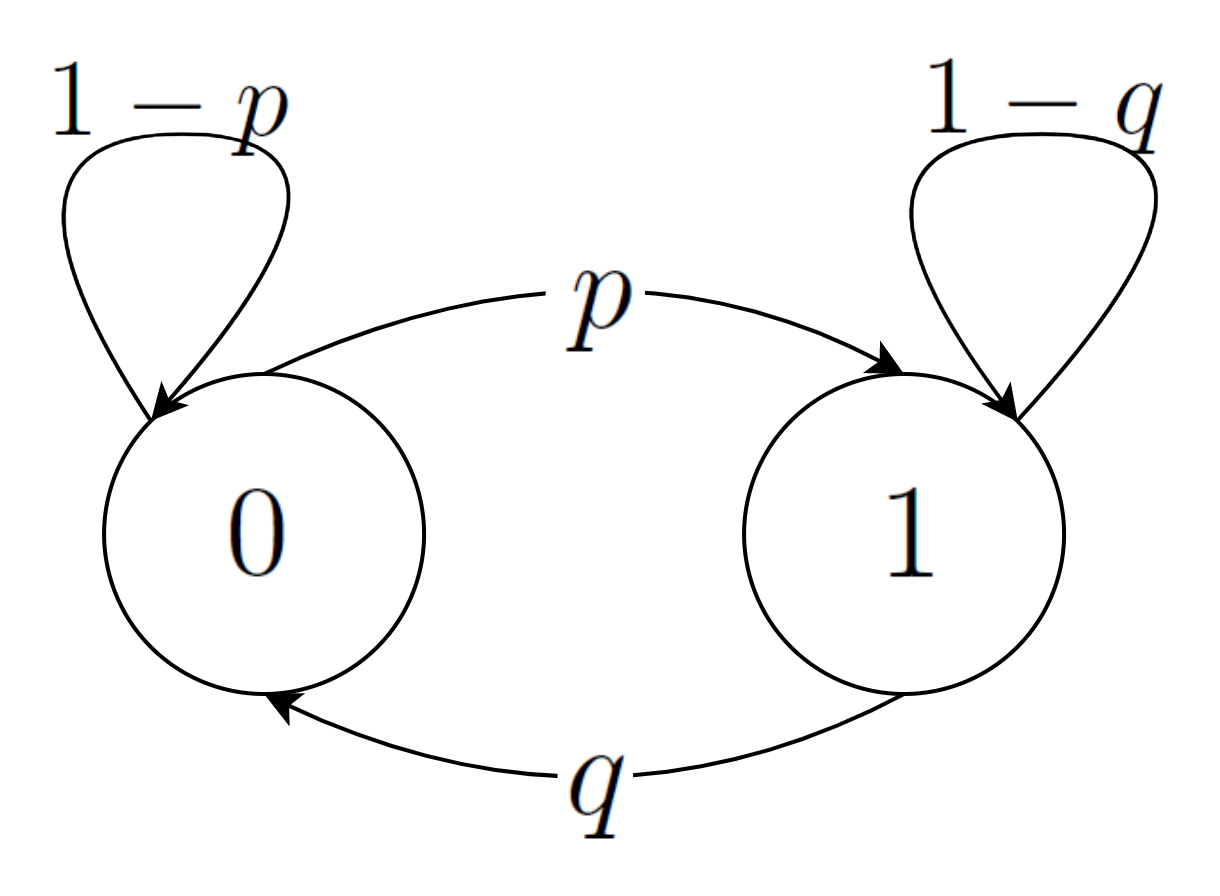
\includegraphics[width=0.4\linewidth]{images/M2.png}
			\caption{Марковская цепь с 2 состояниями}
		\end{figure}
		\begin{equation}P_{\mathcal{M}}(x) = p^{n(01)}\cdot(1-p)^{n(00)}\cdot q^{n(10)}\cdot(1-q)^{n(11)}\to max\end{equation}
		
		\begin{equation}\label{eq:log}\mathcal{L}(\mathcal{M},x)=\log_2{\frac{1}{P_{\mathcal{M}}(x)}}=-(n(01)\cdot\log_2{p}+n(00)\cdot\log_2{(1-p)}+n(10)\cdot\log_2{q}+n(11)\cdot\log_2{(1-q)})\end{equation}
	\end{frame}

	\begin{frame}
		\frametitle{MDL для $\pi$}
		\begin{table}[h]
			\caption{Таблица оптимальных зн-й p и q в двоичной записи для $\pi$}
			\label{table:piBinary}
			\begin{center}
				\begin{tabular}{|l|l|l|l|l|l|l|}
					\hline
					k / l &1 & 2 & 3 & 4 & 5 & 6\\
					\hline
					1 & 31.0& 32.0& 33.0& 33.9891& 34.9521& 35.9521\\
					& 29.0& 29.0& 29.0& 28.9891& 28.9521& 28.9521\\
					& 0.1& 0.1& 0.1& 0.1& 0.1& 0.1\\
					& 0.1& 0.10& 0.100& 0.1001& 0.10001& 0.100010\\
					\hline
					2 & 32.0& 33.0& 34.0& 34.9891& 35.9521& 36.9521\\
					& 29.0& 29.0& 29.0& 28.9891& 28.9521& 28.9521\\
					& 0.10& 0.10& 0.10& 0.10& 0.10& 0.10\\
					& 0.1& 0.10& 0.100& 0.1001& 0.10001& 0.100010\\
					\hline
					3 & 33.0& 34.0& 35.0& 35.9891& 36.9521& 37.9521\\
					& 29.0& 29.0& 29.0& 28.9891& 28.9521& 28.9521\\
					& 0.100& 0.100& 0.100& 0.100& 0.100& 0.100\\
					& 0.1& 0.10& 0.100& 0.1001& 0.10001& 0.100010\\
					\hline
					4 & 34.0& 35.0& 36.0& 36.9891& 37.9521& 38.9521\\
					& 29.0& 29.0& 29.0& 28.9891& 28.9521& 28.9521\\
					& 0.1000& 0.1000& 0.1000& 0.1000& 0.1000& 0.1000\\
					& 0.1& 0.10& 0.100& 0.1001& 0.10001& 0.100010\\
					\hline
					5 & 35.0& 36.0& 37.0& 37.9891& 38.9521& 39.9521\\
					& 29.0& 29.0& 29.0& 28.9891& 28.9521& 28.9521\\
					& 0.10000& 0.10000& 0.10000& 0.10000& 0.10000& 0.10000\\
					& 0.1& 0.10& 0.100& 0.1001& 0.10001& 0.100010\\
					\hline
					6 & 36.0& 37.0& 38.0& 38.9891& 39.9521& 40.9521\\
					& 29.0& 29.0& 29.0& 28.9891& 28.9521& 28.9521\\
					& 0.100000& 0.100000& 0.100000& 0.100000& 0.100000& 0.100000\\
					& 0.1& 0.10& 0.100& 0.1001& 0.10001& 0.100010\\
					\hline
				\end{tabular}
			\end{center}
		\end{table}
	\end{frame}

	\begin{frame}
		\frametitle{}
	\end{frame}
	
\end{document}